
\begin{table}[t]
\centering
\setlength{\tabcolsep}{5pt}
\caption{Effect of the discount factor $\lambda$ of GRPO-DBB on in-distribution Acc@8 performance.
Qwen3-8B-Base achieves the best performance at $\lambda=0.75$, while Qwen3-1.7B-Base performs best at $\lambda=0.5$.}
\label{tab:lambda}
\resizebox{\linewidth}{!}{
    \begin{tabular}{lcccccc>{\columncolor{AvgCol}}c}
    \toprule
    Method & MATH500 & Minerva & AIME24 & AIME25 & AMC24 & Olympiad & Avg. \\
    \midrule
    
    \rowcolor{ModelRow}
    \multicolumn{8}{c}{\textbf{Qwen3-8B-Base} trained with \textbf{DAPO-Math-17k}} \\
    \midrule
    $\lambda = 1.0$
    & 89.08 & 37.91 & 33.33 & 26.25 & 59.44 & 55.19 & 50.20 \\
    $\lambda = 0.75$
    & 88.71 & 39.46 & 33.60 & 29.02 & 60.54 & 56.53 & \textbf{51.31} \\
    $\lambda = 0.5$
    & 89.35 & 38.56 & 33.33 & 27.08 & 59.17 & 56.19 & 50.61 \\
    $\lambda = 0.25$
    & 88.82 & 39.98 & 30.83 & 25.83 & 60.83 & 56.34 & 50.44 \\
    GRPO
    & 87.87 & 39.34 & 29.17 & 25.31 & 57.71 & 54.54 & 48.99 \\
    
    \midrule
    \rowcolor{ModelRow}
    \multicolumn{8}{c}{\textbf{Qwen3-1.7B-Base} trained with \textbf{DAPO-Math-17k}} \\
    \midrule
    $\lambda = 1.0$
    & 67.30 & 25.55 & 9.58 & 3.33 & 23.33 & 28.65 & 26.29 \\
    $\lambda = 0.75$
    & 72.28 & 25.60 & 11.25 & 7.50 & 26.39 & 32.68 & 29.28 \\
    $\lambda = 0.5$
    & 71.67 & 26.43 & 13.75 & 7.40 & 27.31 & 33.36 & \textbf{29.98} \\
    $\lambda = 0.25$
    & 72.22 & 25.97 & 14.17 & 6.25 & 22.50 & 32.88 & 29.00 \\
    GRPO
    & 67.50 & 25.29 & 9.06 & 4.48 & 23.40 & 29.57 & 26.55 \\
    
    \bottomrule
    \end{tabular}
}
\end{table}


\section{Analysis \& Discussion}
In this section, we provide an in-depth analysis of the training behavior and estimation properties of GRPO with the DBB reward estimator.
We first examine training dynamics to understand how DBB influences optimization stability, exploration behavior, and reward progression over time (\cref{subsec:train_dynamics}).
We then conduct ablation studies on the discount factor $\lambda$ to clarify its role in adapting to different learning regimes (\cref{sec:impact_lambda}).
Next, we empirically analyze the mean squared error (MSE) of DBB relative to point estimation, connecting estimation accuracy to downstream performance (\cref{subsec:anal_mse}).
Finally, we demonstrate that DBB can be readily integrated into alternative advantage formulations, highlighting its generality beyond GRPO (\cref{subsec:drgpo}).

% We conduct the following analyses to address the following questions: (1) Why does DBB outperform other baselines? (2) Under what conditions can DBB be effective? (3) Does DBB generalize effectively to RLVR algorithms with alternative advantage formulations?

\subsection{Training Dynamics}
\label{subsec:train_dynamics}

\begin{figure*}[t]
    \centering
    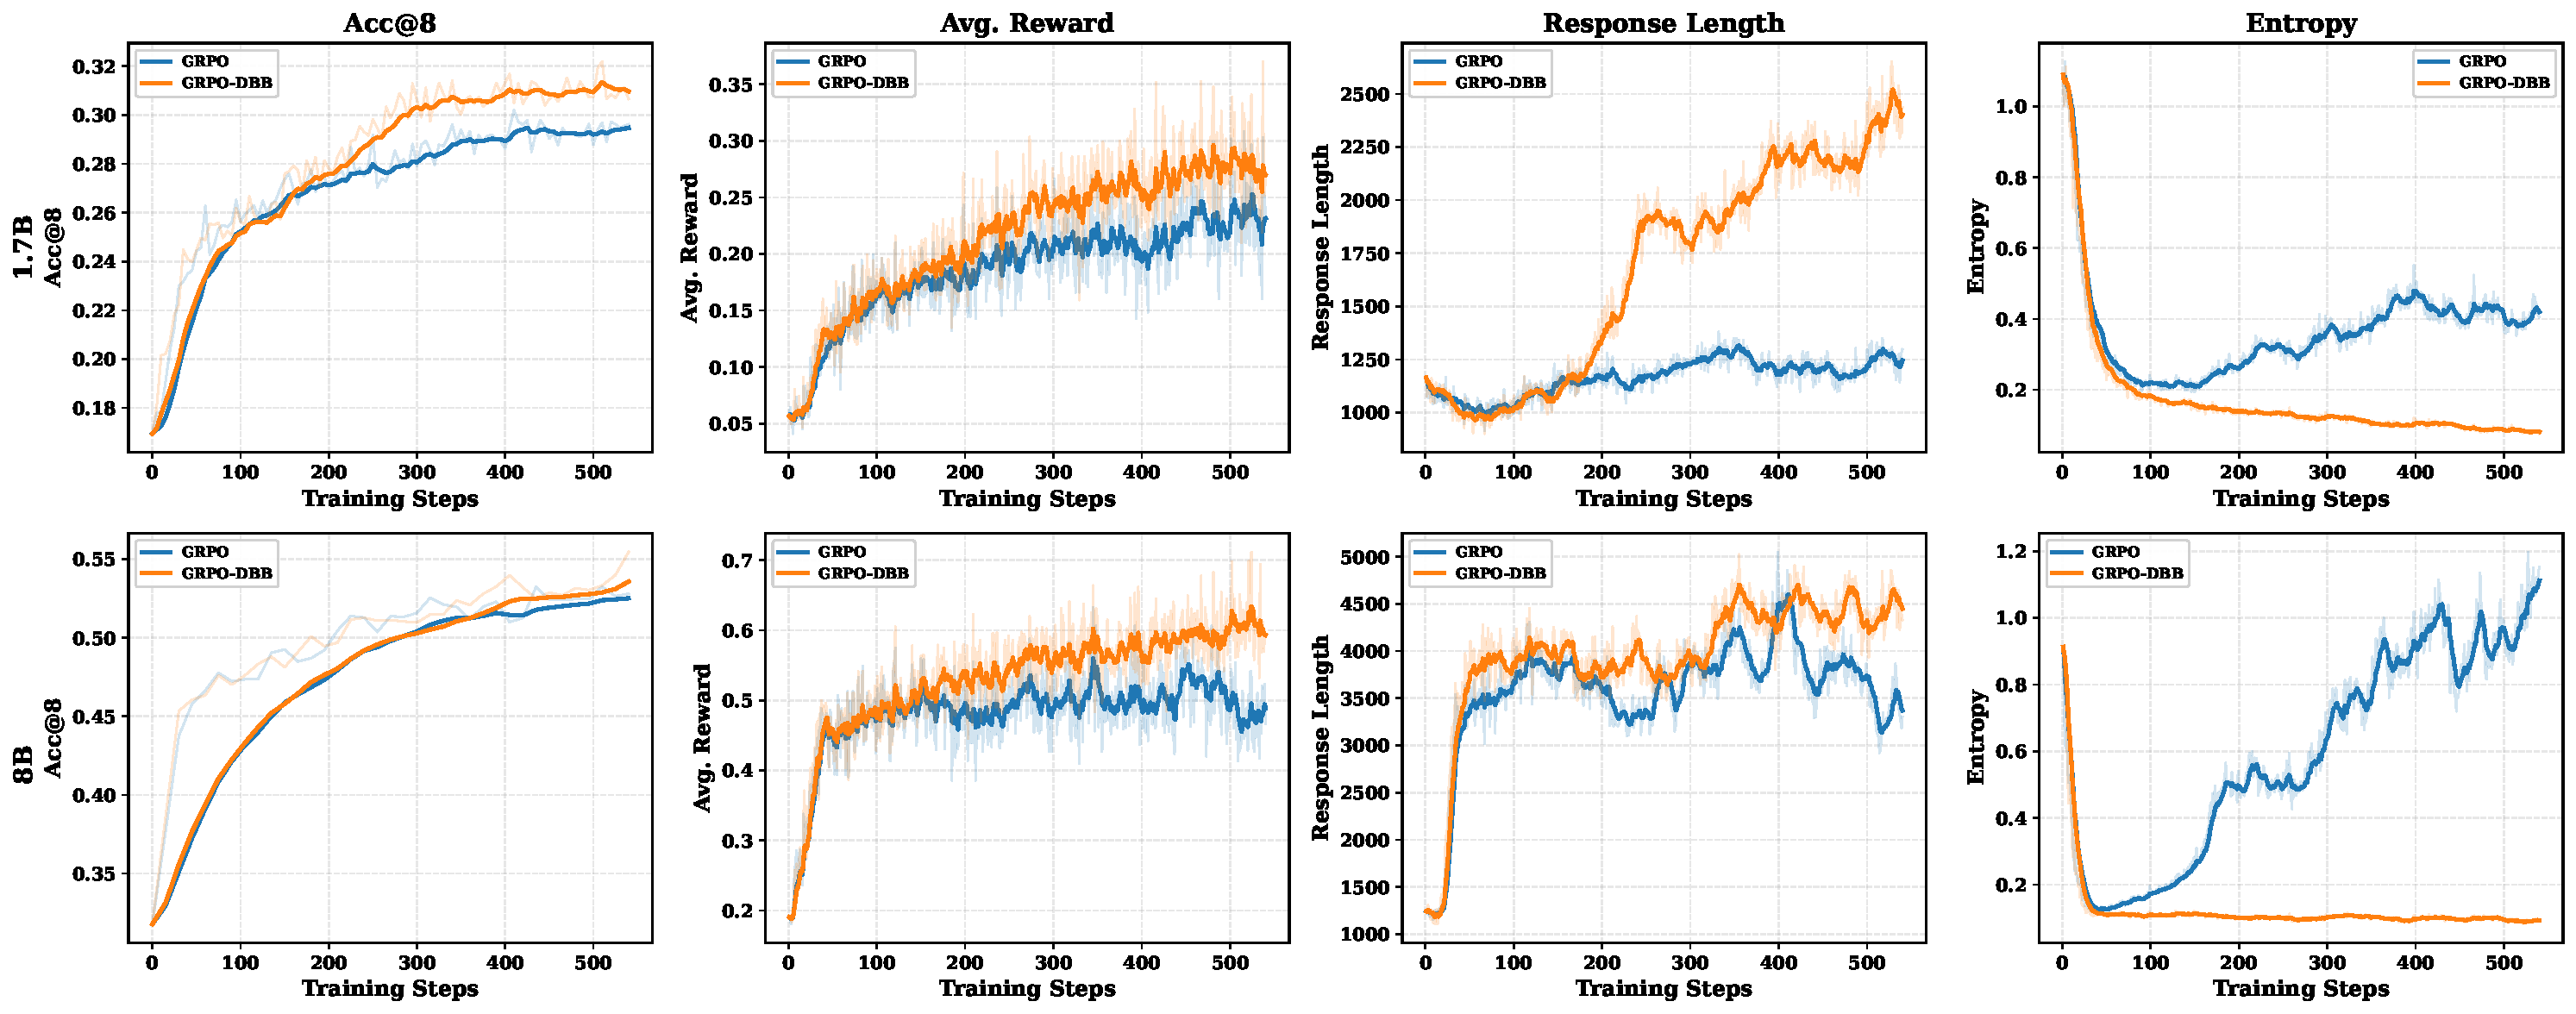
\includegraphics[width=\textwidth]{figures/training_dynamics.pdf}
    \caption{Training dynamics of naive GRPO and GRPO with the DBB estimator (GRPO-DBB) on Qwen3-1.7B-Base (top) and Qwen3-8B-Base (bottom). GRPO-DBB achieves higher validation Acc@8 and training rewards, while maintaining longer responses with controlled entropy compared to GRPO, indicating more stable exploration during training.}
    \label{fig:train_dynamics}
\end{figure*}

Figure~\ref{fig:train_dynamics} illustrates the validation accuracy and training dynamics of GRPO-DBB and GRPO during training.
For GRPO-DBB, the discounting factor $\lambda$ is set to $0.5$ for Qwen3-1.7B-Base and $0.75$ for Qwen3-8B-Base.
For both model scales, GRPO-DBB achieves higher validation accuracy and training rewards than GRPO throughout most of the training process.

Examining the response length over the course of training, we observe that GRPO-DBB consistently produces longer responses than GRPO throughout training.
In contrast, the entropy under GRPO grows rapidly, indicating increasingly unstable exploration behavior.
Taken together, these observations suggest that GRPO-DBB attains higher rewards by pruning the breadth of response trajectories while allowing exploration to proceed along longer trajectories, corresponding to depth-wise exploration.

\paragraph{Why does DBB shrink entropy and elongate responses?}
A decrease in entropy indicates that some token trajectories become less probable and are effectively pruned from the policy's token tree.
This pruning is particularly pronounced for prompts where all sampled rewards within a group are zero.
For such prompts, the group-relative advantage of GRPO collapses to zero and yields no training signal.
In contrast, DBB still produces a non-zero (negative) advantage that rapidly suppresses incorrect trajectories.
We interpret this stronger pruning of zero-variance prompts as a key mechanism underlying the gains of GRPO-DBB.
The increase in response length follows naturally.
To obtain a reward, the model can explore either (i) breadth-wise by diversifying trajectories or (ii) depth-wise by extending them.
Stronger breadth-wise pruning under DBB shifts exploration toward the depth-wise mode, producing significantly longer responses.
Importantly, this lower entropy does not compromise sample diversity at evaluation time.
As shown in Appendix~\ref{ap:best_at_8}, GRPO-DBB matches or exceeds GRPO in Best@8 across both model scales, indicating that meaningful exploratory paths are preserved even as exploration is sharpened.


\subsection{Ablation Study on $\lambda$}
\label{sec:impact_lambda}

To examine the effect of the discount factor $\lambda$ in the DBB estimation, we conduct training experiments of GRPO-DBB with $\lambda = 1.0, 0.75, 0.5,$ and $0.25$ for both model scales.

The hyperparameter $\lambda$ controls the extent to which the estimation of the Bernoulli parameter $p_{\tau}$ for a given query at epoch $\tau$ depends on historical rollout statistics, namely $\alpha_{\tau-1}$ and $\beta_{\tau-1}$.
When the learning dynamics are fast and the discrepancy between $p_{\tau}$ and $p_{\tau-1}$ is large, a smaller $\lambda$ is generally more effective, as it places greater emphasis on recent observations and reduces estimation bias.
Conversely, when the learning dynamics are slower and more stationary, a larger $\lambda$ tends to yield better performance by incorporating more historical information and thereby reducing estimation variance.

This behavior can be interpreted in conjunction with the training reward dynamics shown in Figure~\ref{fig:train_dynamics}.
For Qwen3-1.7B-Base, the training reward exhibits sustained changes throughout the training process, indicating continuously evolving estimates of $p_{\tau}$.
In contrast, for Qwen3-8B-Base, the training reward increases rapidly during the very early stage of training (within approximately the first 0.3 epoch) and remains relatively stationary for the remainder of training.
As a result, a smaller discounting factor ($\lambda = 0.5$) is more effective for Qwen3-1.7B-Base, while a larger value ($\lambda = 0.75$) better matches the slower and more gradual learning dynamics of Qwen3-8B-Base.
More generally, this behavior reflects the bias--variance trade-off of the DBB estimator.
As $\lambda$ increases, variance decreases but bias grows when the reward distribution shifts substantially between epochs.
Weaker models or more challenging datasets tend to incur larger such shifts, making a smaller $\lambda$ preferable.
Conversely, once the model fits the training distribution well, the reward distribution becomes nearly stationary and bounded, so a larger $\lambda$ further reduces MSE.
To corroborate this trend, we additionally conduct a $\lambda$ search on Qwen3-0.6B-Base in Appendix~\ref{ap:lambda_06B}.
There, $\lambda=0.25$ attains the best performance, consistent with the rule of thumb that \emph{smaller models tend to favor smaller $\lambda$}.
Based on this observation, we cautiously suggest a starting point for larger models.
For $30$B$+$ models trained on datasets of similar difficulty to DAPO-Math-17k, $\lambda$ close to $1$ may be a reasonable starting point, while harder datasets are likely to benefit from a smaller $\lambda$.


\label{sec:mse_analysis}
\begin{figure}[t]
    \centering
    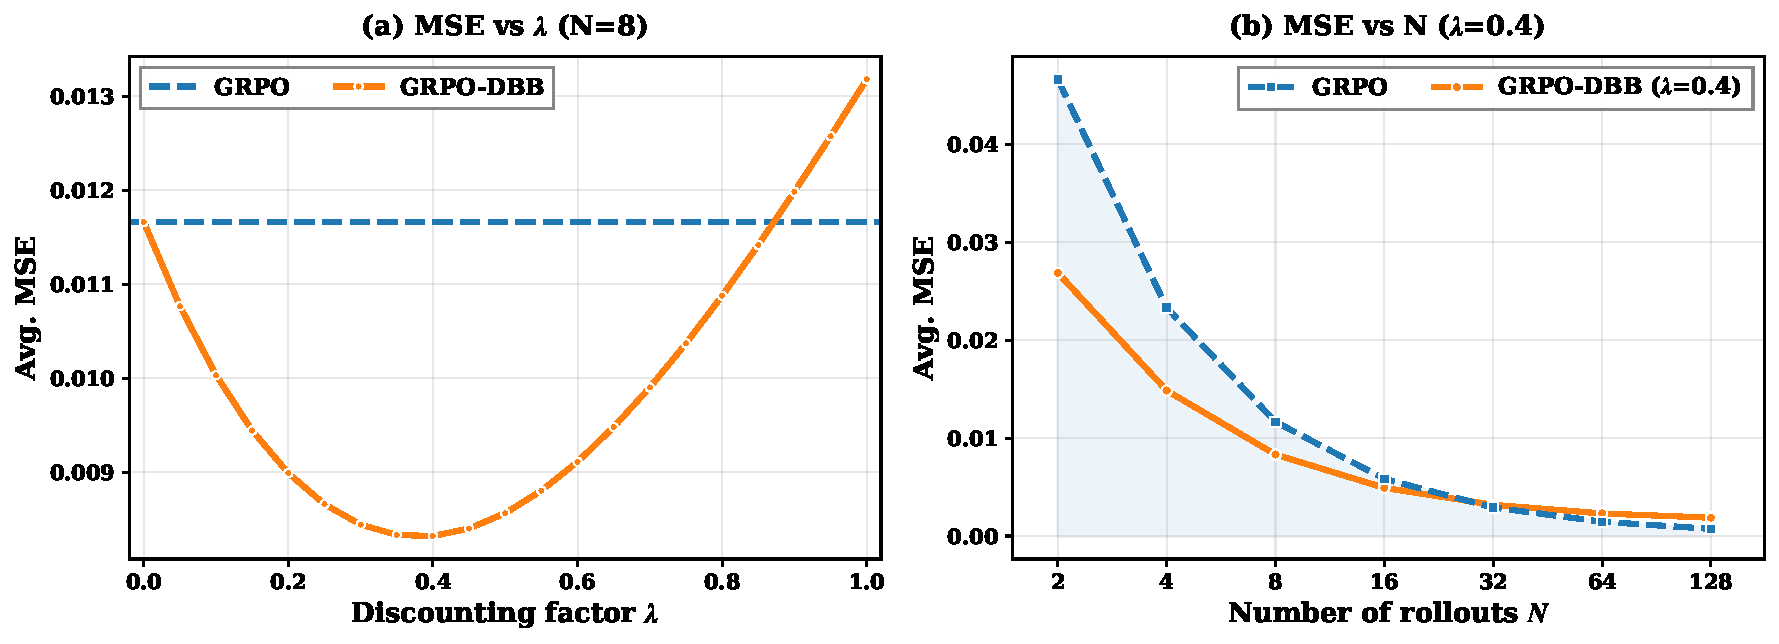
\includegraphics[width=\columnwidth]{figures/mse_combined.pdf}
    \caption{MSE as a function of the discount factor $\lambda$ and the number of rollouts $N$. The DBB estimator yields lower MSE than the point estimator across a wide range of $\lambda$, and it achieves lower MSE for rollout budgets up to $N=16$ when $\lambda=0.4$.}
    \label{fig:mse_lambda}
\end{figure}

\subsection{Analysis of MSE}
\label{subsec:anal_mse}

To evaluate how accurately the point estimator $\hat{p}_{\tau}^{\mathrm{pt}}$ and the DBB estimator $\hat{p}_{\tau}^{\mathrm{dbb}}$ approximate the Bernoulli parameter $p_{\tau}$ during training, we conduct an empirical estimation error analysis.
Since obtaining the exact ground-truth value of $p_{\tau}$ would require infinitely many samples, we instead approximate it using the empirical mean of rewards from a finite number of rollouts.

During GRPO training of Qwen3-1.7B-Base, when a randomly selected 10\% subset of training prompts $\mathcal{Q}_{\tau}$ appears in a rollout batch, we additionally sample 128 responses for each such prompt using the policy at that training step.
These additional samples are used exclusively for analysis and are not incorporated into training.
We then define the empirical mean of the resulting rewards as the reference value $\tilde{p}_{\tau}(q)$.

% \begin{equation}
% \tilde{p}_{\tau}(q)
% \;\triangleq\;
% \frac{1}{128}
% \sum_{i=1}^{128}
% X_{\tau,i},
% \label{eq:ptilde}
% \end{equation}

\vspace{-0.7em}
\begin{equation}
\tilde{p}_{\tau}(q)
\;\triangleq\;
\frac{1}{128}
\sum_{i=1}^{128}
X_{\tau,i},
\label{eq:ptilde}
\end{equation}
\vspace{-0.7em}

\noindent
where
\(
o_{\tau,i} \sim \pi_{\theta_\tau}(\cdot \mid q)
\)
and
\(
X_{\tau,i} = r(o_{\tau,i}, q).
\)
Since training is conducted for a total of four epochs, this procedure yields a sequence of reference values $\{\tilde{p}_{\tau}(q)\}_{\tau=1}^{4}$ for each query.

Using $\tilde{p}_{\tau}(q)$ as a surrogate for the true Bernoulli parameter, we measure the average MSE of the DBB estimator and the point estimator following Equation~\eqref{eq:hb_mse_pseq} and ~\eqref{eq:pt_mse_pseq}, respectively. 


\paragraph{Effect of $\lambda$ on MSE}
\label{subsec:anal_lambda}
Since the value of the DBB estimator depends on the discount factor $\lambda$, we empirically analyze how the MSE varies as a function of $\lambda$.
As shown in Figure~\ref{fig:mse_lambda}(a), the MSE attains its minimum at $\lambda = 0.4$, and for most values of $\lambda$—except for $\lambda = 0.95$ and $\lambda = 1.0$—the DBB estimator yields a lower average MSE than the point estimator.

This trend is closely aligned with downstream performance.
As reported in Table~\ref{tab:lambda}, GRPO-DBB achieves the best performance at $\lambda = 0.5$, while at $\lambda = 1.0$ it performs slightly worse than GRPO with the point estimator.
These observations mirror the behavior of the MSE across different values of $\lambda$.
Taken together, the results indicate that more accurate reward distribution estimation is strongly correlated with improved RLVR performance.

\paragraph{Effect of $N$ on MSE}
We further examine how the MSE varies as the number of rollouts $N$ increases.
Figure~\ref{tab:lambda}(b) reports the average MSE as a function of $N$ when $\lambda = 0.4$.
The results show that the DBB estimator consistently outperforms the point estimator for $N$ up to 16.
This suggests that, in regimes where computational resource constraints necessitate small rollout budgets, the DBB estimator can serve as an effective alternative to point estimation.

\paragraph{Comparison with simpler shrinkage estimators}
We further benchmark DBB against per-prompt exponential moving average (EMA) and per-prompt Laplace smoothing as simpler shrinkage baselines.
As detailed in Appendix~\ref{ap:ema_laplace}, DBB attains the lowest minimum MSE and improves on the point estimator over a broader $\lambda$ range than either alternative, supporting our choice of the DBB estimator over light-weight shrinkage alternatives.

\subsection{Evaluation on Alternative Advantage Formulations}
\label{subsec:drgpo}
\begin{table}[t]
\centering
\setlength{\tabcolsep}{5pt}
\caption{In-distribution evaluation results on Qwen3-1.7B-Base trained with DAPO-MATH-17k.
We apply the proposed discounted Beta--Bernoulli reward distribution estimation to the advantage term of Dr.GRPO and observe consistent performance improvements.
$\Delta$ denotes the absolute Acc@8 improvement over naive Dr.GRPO.}
\label{tab:drgrpo}
\resizebox{\linewidth}{!}{
    \begin{tabular}{lcccccc>{\columncolor{AvgCol}}c}
    \toprule
    Method & MATH500 & Minerva & AIME24 & AIME25 & AMC24 & Olympiad & Avg. \\
    \midrule
    
    \rowcolor{ModelRow}
    \multicolumn{8}{c}{\textbf{Qwen3-1.7B-Base} trained with \textbf{DAPO-Math-17k}} \\
    \midrule
    Dr.GRPO
    & 69.00 & 25.14 & 9.17 & 7.92 & 23.89 & 32.78 & 27.98 \\
    \midrule
    Dr.GRPO-DBB
    & \textbf{70.60} & \textbf{26.15} & \textbf{12.08} & \textbf{9.17} & \textbf{28.06} & \textbf{33.59} & \textbf{29.94} \\
    $\Delta$ w.r.t.\ Dr.GRPO
    & \textbf{+1.60} & \textbf{+1.01} & \textbf{+2.92} & \textbf{+1.25} & \textbf{+4.17} & \textbf{+0.81} & \textbf{+1.96} \\
    
    \bottomrule
    \end{tabular}
}
\end{table}

To examine whether the DBB estimation can be applied to other advantage formulations, we conduct experiments using the advantage term of Dr.GRPO, defined as $A_i = X_i - \mathbb{E}[\hat{p}_\tau]$.
All experiments are conducted on Qwen3-1.7B-Base with the discounting factor set to $\lambda = 0.5$ for the Dr.GRPO with the DBB estimation (Dr.GRPO-DBB).
As shown in Table~\ref{tab:drgrpo}, Dr.GRPO-DBB consistently improves performance over the naive Dr.GRPO across all in-distribution benchmarks, yielding an average Acc@8 gain of 1.96 points.
These results suggest that the DBB estimation is not limited to the advantage term of GRPO, but can be broadly applied to other RLVR algorithms that rely on point estimation, yielding effective and consistent performance gains.
